\sect{Metodología de trabajo}{metodologia}

Para el desarrollo de la aplicación se ha utilizado el marco de trabajo \boldFont{SCRUM}, que se emplea para la gestión
de proyectos ágiles de manera \boldFont{iterativa} e \boldFont{incremental}~\cite{scrum:book}.
Iterativa porque se revisa y mejora
el producto existente en cada ciclo de desarrollo (\boldFont{sprint}), e incremental porque las nuevas
funcionalidades se integran en la aplicación a medida que se completan.

Todas las funcionalidades a implementar se
denominan \boldFont{historias de usuario} y forman lo que se denomina Pila del Producto (\boldFont{Product Backlog}).
En cada iteración, se seleccionan las historias de usuario que se consideran más prioritarias y se asignan a los
miembros del equipo de trabajo, formando la Pila del Sprint (\boldFont{Sprint Backlog}).

La duración de las iteraciones en SCRUM es variable, pero se recomienda que no sea inferior a 2 semanas.\ En este
proyecto se ha optado por una duración de 4 semanas, ya que el tiempo de desarrollo de cada iteración debe ser
suficiente para que el desarrollador pueda completar todas las tareas que se le han asignado durante la misma.

Puesto que el equipo de trabajo está formado por un único miembro, no ha sido necesario realizar reuniones de
coordinación, porque se ha podido trabajar de manera autónoma y sin necesidad de supervisión.\ Además, se ha
adaptado el marco de trabajo para que se ajuste a las necesidades del proyecto.

La gestión de la pila del producto se ha realizado con la herramienta \boldFont{Notion}, que permite crear espacios
de trabajo con diferentes vistas para organizar las tareas.\ En la figura~\ref{fig:notion-product-backlog} se presenta
una pequeña muestra de la pila del producto.\ Para una descripción más detallada y completa de las tareas realizadas
durante el desarrollo del proyecto, se puede consultar el anexo~\ref{anx:product-backlog-notion}.

\begin{figure}[H]
	\centering
	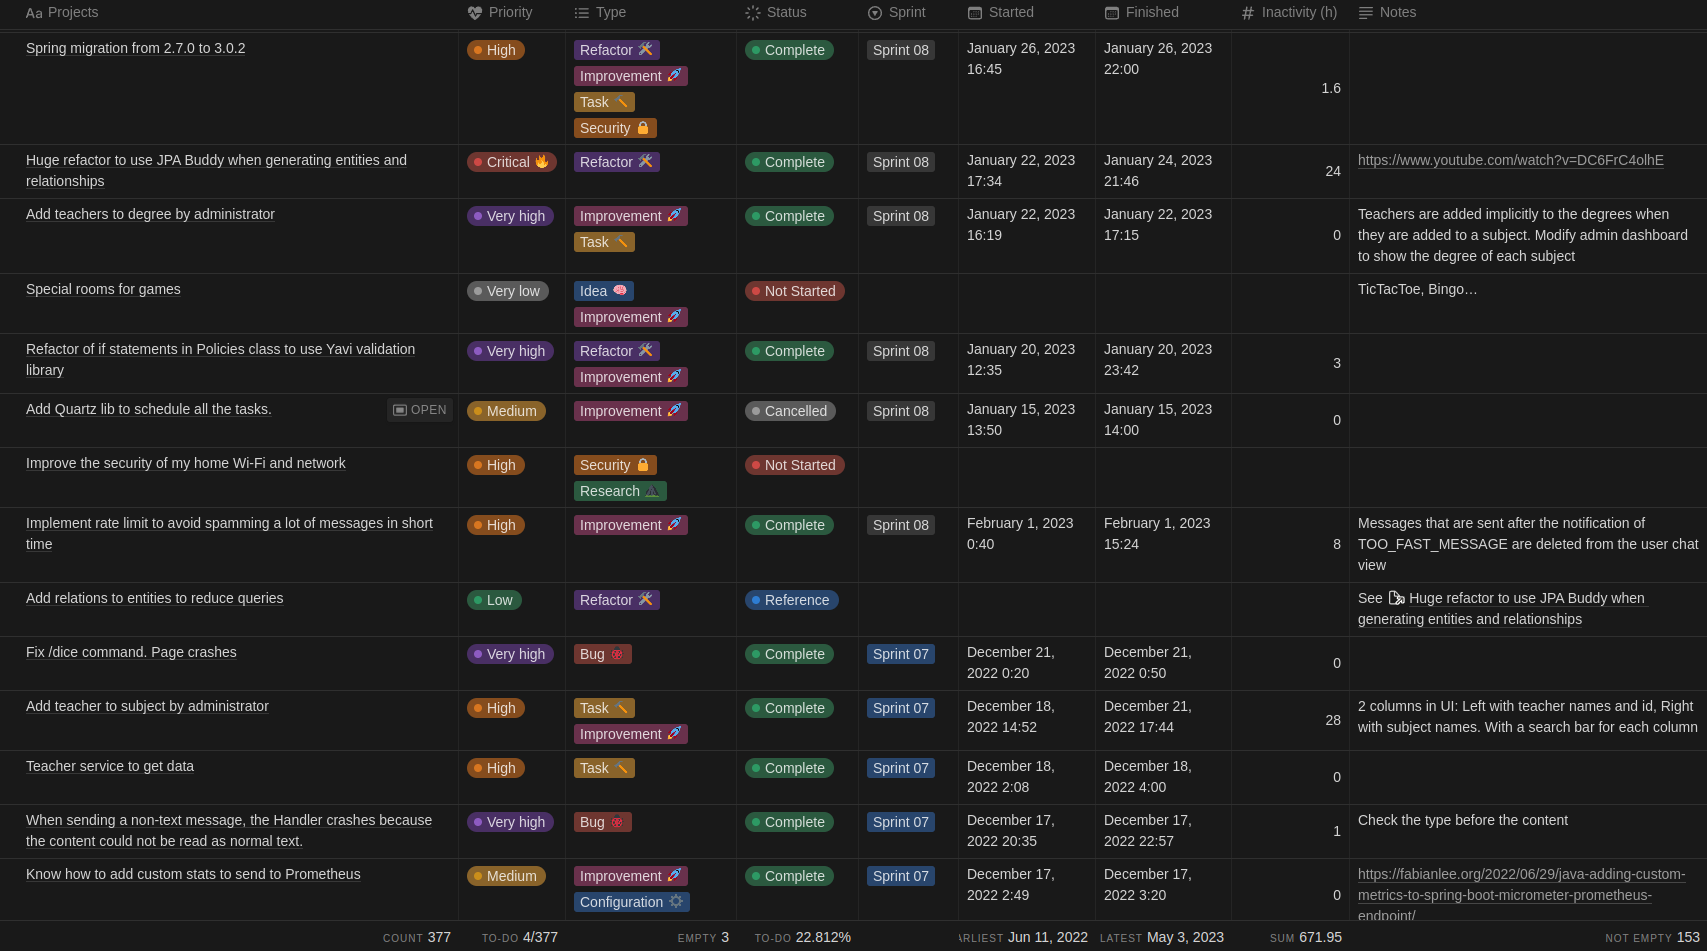
\includegraphics[width=\textwidth]{notion-product-backlog}
	\caption{Pila del producto en Notion}
	\label{fig:notion-product-backlog}
\end{figure}
